%\subsection{Coordinate Capture Plugin}
\subsection{Extension de saisie de coordonn\'es}

% when the revision of a section has been finalized, 
% comment out the following line:
% \updatedisclaimer

%The coordinate capture plugin is easy to use and provides the 
%capability to display coordinates on the map canvas for two 
%selected Coordinate Reference Systems (CRS). You can click a 
%certain point and copy the coordinates to the clipboard or you 
%use the mouse tracking functionality.

L'extension saisie de coordonn\'es, facile \`a utiliser, permet 
d'afficher des coordonn\'es sur la carte pour deux syst\`emes de 
coordonn\'es de r\'ef\'erence (CRS) s\'electionn\'es. Vous pouvez cliquer 
sur un point et copier les coordonn\'es dans le presse-papier, ou 
utiliser la fonction de suivi de la souris.

%\begin{figure}[ht]
%   \begin{center}
%   \caption{Coordinate Cature Plugin \nixcaption}\label{fig:coordinate_capture_dialog}\smallskip
%   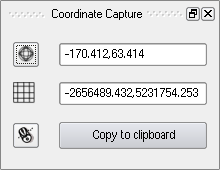
\includegraphics[clip=true]{coordinate_capture_dialog}
%\end{center}  
%\end{figure}

\begin{figure}[ht]
   \begin{center}
   \caption{L'extension Saisie de Coordonn\'es \nixcaption}\label{fig:coordinate_capture_dialog}\smallskip
   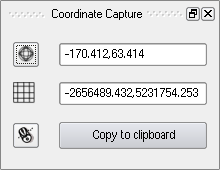
\includegraphics[clip=true]{coordinate_capture_dialog}
\end{center}  
\end{figure}

%\begin{enumerate}
%  \item Start QGIS, select \dropmenuopttwo{mActionOptions}{Project Properties} from 
%  the \mainmenuopt{Settings} menu and click on the \tab{Projection} tab. As an alternative you 
%  you can also click on the \toolbtntwo{mIconProjectionEnabled}{projector} icon in the lower 
%  right-hand corner of the statusbar.
%  \item Click on the \checkbox{Enable on the fly projection} checkbox and select the projected 
%  coordinate system \filename{"NAD27/Alaska Albers"} with EPSG 2964 (see also 
%  Section \ref{label_projections}).
%  \item Load the \filename{alaska.shp} vector layer from the qgis sample dataset.
%  \item Load the coordinate capture plugin in the Plugin Manager (see Section 
%  \ref{sec:load_core_plugin}) and click on the \toolbtntwo{coordinate_capture}{Coordinate Capture} 
%  icon. The cordinate capture dialog appears as shown in Figure \ref{fig:coordinate_capture_dialog}.
%  \item Click on the \toolbtntwo{geographic}{Click to the select the CRS to use for coordinate %display} 
%  icon and select Geographic Coordinate System \filename{WGS84} (EPSG 4326).
%  \item You can now click anywhere on the map canvas and the plugin will show the 
%  \filename{"NAD27/Alaska Albers"} and \filename{WGS84} coordinates for your selected points as %shown in 
%  Figure \ref{fig:coordinate_capture_dialog}.
%  \item To enable mouse coordinate tracking click the \toolbtntwo{tracking}{mouse tracking} icon.
%  \item You can also copy selected coordinates to the clipboard.
%\end{enumerate}

\begin{enumerate}
  \item D\'emarrez QGIS, s\'electionnez \dropmenuopttwo{mActionOptions}{Propri\'et\'es du Projet} du menu
  \mainmenuopt{Pr\'ef\'erences} et cliquez sur l'onglet \tab{Syst\`eme de coordonn\'es de pr\'ef\'erence (CRS)}. 
  Il est \'egalement possible de cliquer sur l'ic\^one \toolbtntwo{mIconProjectionEnabled}{Statut de la
  projection}, dans le coin bas droite de la barre de statut.
  \item Cochez l'option \checkbox{Autoriser la projection '\`a la vol\'ee'} et s\'electionnez le syst\`eme
  de coordonn\'es projet\'e \filename{"NAD27/Alaska Albers"} dont l'EPSG est 2964 (voir aussi 
  la Section \ref{label_projections}).
  \item Chargez la couche vecteur \filename{alaska.shp} depuis le jeu de donn\'ees \'echantillon de QGIS.
  \item Chargez l'extension Saisie de coordonn\'es dans le Gestionnaire d'extensions (voir la Section
  \ref{sec:load_core_plugin}) et cliquez sur l'ic\^one \toolbtntwo{coordinate_capture}{Saisie de coordonn\'es}.
  Une bo\^ite de dialogue appara\^it, comme indiqu\'e dans la Figure \ref{fig:coordinate_capture_dialog}.
  \item Cliquez sur l'ic\^one \toolbtntwo{geographic}{Cliquez ici pour s\'electionner le SRS \`a utiliser pour l'affichage 
  des coordonn\'es} et s\'electionnez le Syst\`eme de coordonn\'es G\'eographiques \filename{WGS84} (EPSG 4326).
  \item Vous pouvez d\'esormais cliquer n'importe o\`u dans la fen\^etre carte et les coordonn\'es des points 
  s\'electionn\'es s'afficheront en \filename{"NAD27/Alaska Albers"} et \filename{WGS84}, comme indiqu\'e dans la
  Figure \ref{fig:coordinate_capture_dialog}.
  \item Pour activer le suivi des coordonn\'es du curseur de la souris, cliquez sur l'ic\^one \toolbtntwo{tracking}{suivi du curseur}.
  \item Vous pouvez \'egalement copier les coordonn\'es vers le presse-papiers.
\end{enumerate}

\newpage